\chapter{Caracterização da Amostra}
\label{chap:result}

% Neste capítulo são apresentados os resultados obtidos da pesquisa e sua análise. Primeiramente é aprestada uma síntese dos dados da amostra coletada com o \textit{survey} e uma análise sobre eles. E por fim são apresentadas as personas e uma análise de como elas refletem a amostra. 

Neste capítulo é apresentada a caracterização, análise e discussão dos resultado da amostra em relação ao perfil dos usuários de jogos em IHC. São abordadas as características demográficas; as motivações no uso de jogos para aprendizagem; interação com meios para aprendizagem em IHC; relação dos alunos com jogos para aprendizagem; experiência do jogador em design; e os aspectos de qualidade em jogos para aprendizagem.

\section{Características Demográficas}

% I01; I02; I03; I04

Em relação às características demográficas da amostra, a idade dos respondentes varia entre 18 e 53 anos, sendo que 75\% deles possuem até 23 anos de idade. Em relação ao sexo, 128 respondentes (77\%) são do sexo masculino, 36 (22\%) do sexo feminino, um dos respondentes preferiu não responder a essa pergunta (0.5\%) e ainda um outro respondentes selecionou outro sexo como resposta (0.5\%), mas sem citar qual.

Dentre as instituições de ensino que participaram da pesquisa, foram obtidas 126 respostas de alunos e ex-alunos da UnB (76\%), 24 da UFMS (14\%), 10 da UFAM (6\%), 4 da UFMT (2\%), 1 da UCSAL (0.5\%) e outra da UTFPR (0.5\%). Todos os respondentes válidos cursavam ou cursaram graduação em alguma áreas da Ciência da Computação.

Pode-se perceber que grande parte da amostra são jovens adultos entre 18 e 23 anos, sendo a maior parte do sexo masculino, graduandos em algum curso da área de Ciência da Computação a UnB.

\section{Motivações no Uso de Jogos para Aprendizagem}

% Variável O01;  
Quanto à motivação de uso dos jogos para aprendizagem, foi primeiramente observado que em relação à disciplina de Interação Humano-Computador (IHC), 65 respondentes (39\%) estavam fazendo a disciplina, 57 respondentes (34\%) já haviam feito e 44 (27\%) não haviam feito a disciplina de IHC. A Figura \ref{Fig:rel-disc-ihc.png} apresenta estes dados.

\begin{figure}[htbp]
	\centering
	\caption{Relação de Respondentes com a Disciplina de IHC}
	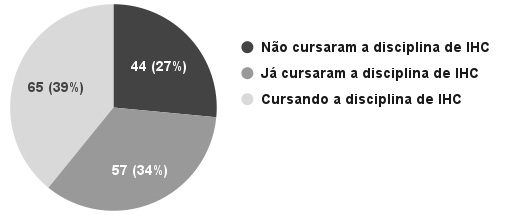
\includegraphics[keepaspectratio=true,scale=0.65]{figuras/resultados/rel-disc-ihc.png}
	\legend{Fonte: Própria Autoria}
	\label{Fig:rel-disc-ihc.png}
\end{figure}

Como pode-se perceber na Figura \ref{Fig:rel-disc-ihc.png}, a amostra está bem distribuída. Esta relação entre os aluno e sua posição quanto à disciplina de IHC foi analisada em vista das motivações de uso dos jogos para aprendizagem. 

% Variável O02.1.1; O02.2.1; O02.3.1;
Cada respondente pôde apresentar um ou mais motivos para usar esse tipo de jogo. A Figura \ref{Fig:obj-estudo.png} apresenta estas motivações.

\begin{figure}[htbp]
	\centering
	\caption{Relação de Respondentes com suas Motivações de Estudo}
	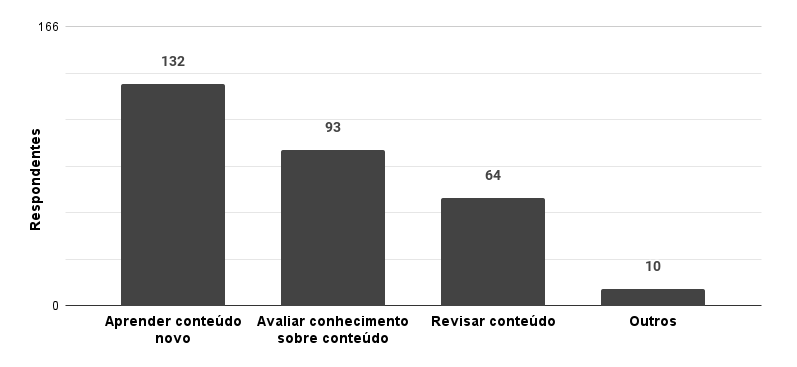
\includegraphics[keepaspectratio=true,scale=0.55]{figuras/resultados/obj-estudo.png}
	\legend{Fonte: Própria Autoria}
	\label{Fig:obj-estudo.png}
\end{figure}

Dentre as motivações de uso dos jogos observou-se que 132 respondentes possuem a intenção em aprender um novo conteúdo (Figura \ref{Fig:obj-estudo.png}), ou seja, 79\% visavam pelo menos esse objetivo; 93 respondentes demonstraram que possuíam interesse de avaliar o nível de conhecimento com esse tipo de jogo (Figura \ref{Fig:obj-estudo.png}), ou seja, 56\% tinham pelo menos essa motivação; e 64 respondentes revelaram possuir como motivo, ao menos revisar um conteúdo já aprendido através de jogos (Figura \ref{Fig:obj-estudo.png}), sendo estes 38\% dos respondentes. 

Além destes, 10 respondentes (6\%) apontaram outros motivos para se usar esse tipo de jogo (Figura \ref{Fig:obj-estudo.png}). As motivações foram, a busca por diversão, curiosidade, lazer e entretenimento. Outros relataram que apenas jogaram algo do tipo pelo fato de ter sido uma atividade acadêmica. 

Três foram as motivações que se destacaram (Figura \ref{Fig:obj-estudo.png}). Elas foram analisadas em relação à posição do aluno com a disciplina de IHC, conforme apresentado na Figura \ref{Fig:rel-disc-obj.png}.

\begin{figure}[htbp]
	\centering
	\caption{Relação das motivações de estudo e a posição dos alunos na disciplina de IHC}
	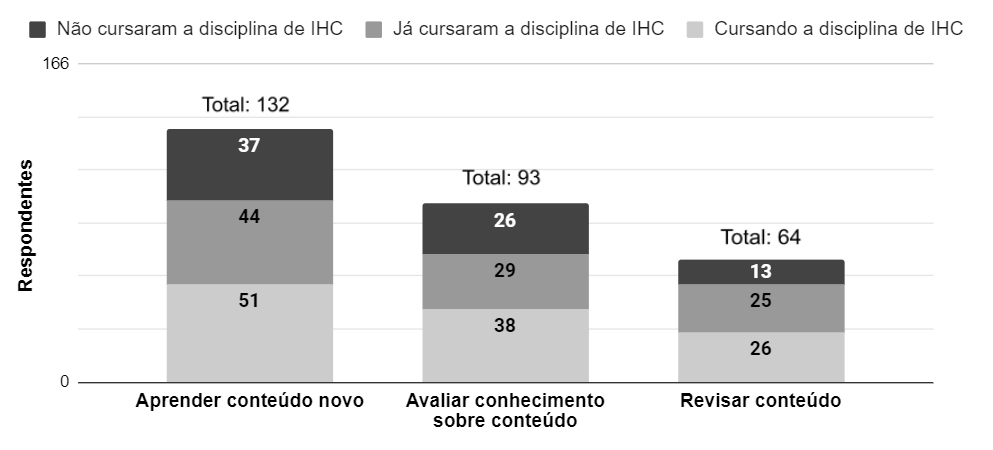
\includegraphics[keepaspectratio=true,scale=0.55]{figuras/resultados/rel-disc-obj.png}
	\legend{Fonte: Própria Autoria}
	\label{Fig:rel-disc-obj.png}
\end{figure}

Dos 44 respondentes que ainda não tinham feito a disciplina de IHC (Figura \ref{Fig:rel-disc-ihc.png}), 37 desejavam pelo menos usar os jogos para aprender um conteúdo novo; 26 gostariam de ao menos avaliar seu conhecimento; e houveram 13 respondentes que tinham como motivação revisar um conteúdo com o uso de jogos (porções superiores de cada barra na Figura \ref{Fig:rel-disc-obj.png}). Dos 57 que já haviam feito a disciplina (Figura \ref{Fig:rel-disc-ihc.png}), 44 gostariam de no mínimo aprender um conteúdo novo através de jogos; 29 tinham ao menos o interesse de avaliar seu conhecimento; e 25pelo menos revisar um conteúdo já aprendido (porção do meio de cada barra na Figura \ref{Fig:rel-disc-obj.png}). Dos 65 alunos que estavam cursando IHC (Figura \ref{Fig:rel-disc-ihc.png}), 51 tinham pelo menos o interesse de aprender um novo conteúdo; 38 pelos menos gostariam de avaliar seu conhecimento; e 27 gostariam de ao menos revisar o conteúdo através de jogos (porção inferior de cada barra na Figura \ref{Fig:rel-disc-obj.png}).

A motivação mais frequente foi o de aprender um conteúdo novo através dos jogos para aprendizagem. Esta característica do perfil do jogador se destaca mais quando ligada ao fato de que a maioria dos respondentes estavam cursando a disciplina de IHC. Ou seja, os alunos que desejam aprender um conteúdo novo com jogos e cursam IHC (51 respondentes, Figura \ref{Fig:rel-disc-obj.png}) são usuários em potencial para usar esse tipo de jogo na introdução dos conceitos desta disciplina. 

Da semelhante forma, 37 alunos que não cursaram a disciplina de IHC, mas que tinham o interesse de aprender um conteúdo por meio de jogos (Figura \ref{Fig:rel-disc-obj.png}) são candidatos a usuários de jogos em IHC. Estes, quando fossem cursar a disciplina seriam possíveis usuário desse tipo de jogo, tendo a motivação de aprenderem o conteúdo de IHC.

Outra parcela da amostra que merece destaque, são os alunos que estavam cursando a disciplina de IHC. Estes 38 destacam-se por desejarem usar jogos para avaliar seu conhecimento sobre um conteúdo (Figura \ref{Fig:rel-disc-obj.png}). Eles também são um perfil de jogadores em potencial, no entanto usariam esse tipo de jogo após aprenderem o conteúdo, avaliando então o que aprenderam.

Por fim, destacam-se aqueles que já haviam cursado a disciplina de IHC e tinham o interesse em aprender um conteúdo novo (44 respondentes, Figura \ref{Fig:rel-disc-obj.png}). Estes não se enquadram no perfil do jogador-alvo para jogos em IHC. No caso, estes poderiam representar um outro tipo de usuário dentro do jogo, já que não haveria o interesse em aprender IHC. 

Estas foram as motivações mais relevantes identificadas, tendo em vista a definição de um perfil de jogador-alvo. As demais relações entre as motivações dos alunos e sua posição quanto à disciplina de IHC que foram analisadas não foram consideradas por não apresentarem tanta relevância quanto as demais. Porém estas motivações podem até representar usuários excepcionais que busquem usar jogos para a aprendizagem em IHC.

\section{Interação com Meios para Aprendizagem em IHC}

Cada aluno ainda apresentou um ou mais meios pelos quais eles tiravam suas dúvidas nas disciplinas acadêmicas. A Figura \ref{Fig:rel-rel.png} apresenta os meios utilizados pelos alunos como suporte ao processo de aprendizagem. 

%RL01
\begin{figure}[htbp]
	\centering
	\caption{Meios para Aluno Sanar as dúvidas}
	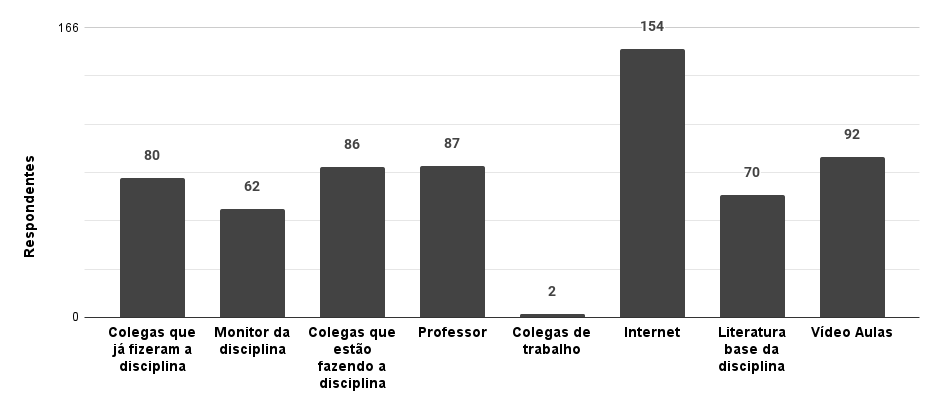
\includegraphics[keepaspectratio=true,scale=0.485]{figuras/resultados/rel-rel.png}
	\legend{Fonte: Própria Autoria}
	\label{Fig:rel-rel.png}
\end{figure}

Dentre estes meios de se tirar dúvida, observa-se na Figura \ref{Fig:rel-rel.png}, que 80 dos respondentes buscavam sanar suas dúvidas com algum colega que que já haviam feito a disciplina (48\%); 86 foram os que buscaram suporte com colegas que cursavam a disciplina no mesmo período (51\%); e 62 optaram por pedir ajuda ao monitor da disciplina (37\%); e 87 iam tirar dúvidas com o professor (52\%). Em média 47\% dos alunos buscavam interagir com outras pessoas do próprio meio acadêmico para sanar suas dúvidas sobre alguma disciplina do curso. Ainda outro meio pessoal pelo qual 2 respondentes apontaram ser uma forma de tirar dúvidas, foi com os colegas de trabalho (1\%).

Já em relação aos meios não pessoais (Figura \ref{Fig:rel-rel.png}), observa-se que 154 respondentes buscavam na Internet (artigos, blogs, revistas científicas por exemplo) a solução de suas dúvidas (93\%); 70 buscavam na própria literatura sugerida na ementa da disciplina (42\%) e 92 assistiam video-aulas para sanar suas dúvidas (55\%). Nota-se que há uma tendência maior dos alunos em buscarem informações para sanar as dúvidas através dos recursos disponíveis na internet do que em outros meios. 

Pensando nisto, um usuário de jogos para aprendizagem com este perfil, teria maior preferencia por jogos que ao apresentar um conteúdo apontassem para um material online mais completo, o qual o usuário pudesse estudar mais a fundo o conteúdo caso fosse necessário. Isso não descartaria funcionalidades de fóruns de dúvidas ou outros meios de interação entre outros usuários do jogo, mas estes não seriam recursos prioritários.

\section{Relação dos Alunos com Jogos para Aprendizagem}
% variável O02;
Esta análise inicial somada à interação que estes alunos já tiveram com jogos para aprendizagem traz mais informações relevantes para caracterização da amostra em relação a elaboração de um perfil de usuários de jogos em IHC. A Figura \ref{Fig:uso-jogo.png} apresenta a relação entre respondentes e sua interação com jogos para aprendizagem.

\begin{figure}[htbp]
	\centering
	\caption{Interação dos alunos com jogos para aprendizagem}
	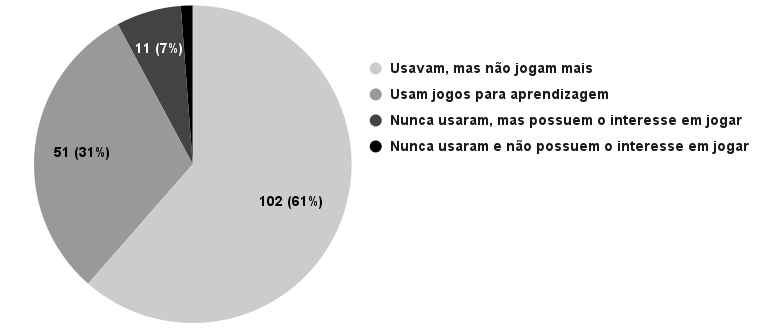
\includegraphics[keepaspectratio=true,scale=0.5]{figuras/resultados/uso-jogo.png}
	\legend{Fonte: Própria Autoria}
	\label{Fig:uso-jogo.png}
\end{figure}

% O02.3.2 e O02.4.1
Em relação à interação dos respondentes com jogos para aprendizagem, foi identificado que 102 (61\%) já usaram algum jogo, mas não jogavam mais (Figura \ref{Fig:uso-jogo.png});  51 respondentes (31\%) ainda usavam jogos para aprender algum conteúdo (Figura \ref{Fig:uso-jogo.png}); e 13 respondentes nunca haviam usado esse tipo de jogo. 

Destes 13 respondentes que nunca haviam usado jogos para aprendizagem, 11 tinham o interesse em jogá-los (7\%), mas por não conhecerem jogos sobre o conteúdo desejado, nunca haviam jogado (Figura \ref{Fig:uso-jogo.png}). Já os outros 2 não tinham interesse nesse tipo de jogo (1\%), por não considerarem que jogos pudessem ser um recurso no processo de aprendizagem (Figura \ref{Fig:uso-jogo.png}).

Pôde-se notar que grande parte dos respondentes já haviam tido alguma interação com jogos para aprendizagem e daqueles que não tinham tido essa interação, haviam alguns com interesse em usá-los. Isso reforça a busca que há no meio acadêmico por recursos inovadores para auxiliar o ensino e aprendizagem \cite{battistella,brito,Sales2020,Sales2020UsoTDS}.

% O02.1.4
Dentre estes 102 respondentes que deixaram de usar algum jogo para aprendizagem, pôde ser observado suas motivações. Cada respondente relatou um ou mais motivos que os levaram a deixar de jogar esse tipo de jogo. A Figura \ref{Fig:deixa-jogo.png} apresenta estes dados.

\begin{figure}[htbp]
	\centering
	\caption{Motivações dos alunos que deixaram de usar jogos para aprendizagem}
	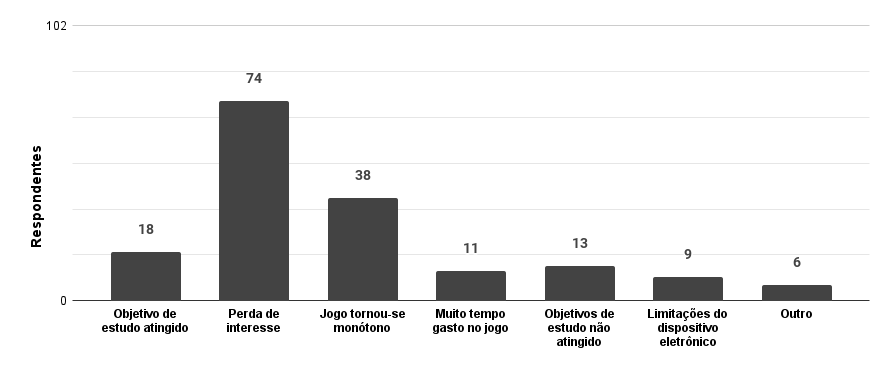
\includegraphics[keepaspectratio=true,scale=0.5]{figuras/resultados/deixa-jogo.png}
	\legend{Fonte: Própria Autoria}
	\label{Fig:deixa-jogo.png}
\end{figure}

Das motivações dos usuários que deixaram de utilizar esse tipo de jogo, pode ser observado na Figura \ref{Fig:deixa-jogo.png}, que alguns perderam o interesse no jogo, 74 respondentes (73\%); alguns relataram que o jogo se tornou monótono, 38 respondentes (37\%); já 18 respondentes (18\%) afirmaram ter conseguido alcançar seu objetivo de estudo com o jogo; porém outros deixaram de usar estes jogos por não terem alcançado seu objetivo de estudo, 13 respondentes (13\%); e 11 (11\%) relataram gastar tempo demais com estes jogos.

Ainda 9 respondentes (9\%) relataram que tiveram problemas com o dispositivo eletrônico, como memória cheia ou atualizações que impossibilitaram o uso do jogo no dispositivo; e 6 respondentes (6\%) apresentaram outros motivos, como a necessidade de outros recursos para complementar o estudo, não encontrar mais espaço na rotina para usar o jogo e ter percebido que o jogo não era um método que se adequava ao seu perfil.

Sendo que apenas 18 usuário atingiram seu objetivo de estudo através de jogos, pode-se perceber que 82\% dos respondentes que usaram algum jogo para aprendizagem deixaram de usá-los por uma motivação negativa em relação ao jogo, salvo aqueles que tiveram problemas com seus dispositivos eletrônicos. Ou seja, grande parte dos jogadores não alcançaram seus objetivos de estudo com o uso deste tipo de jogo por conta dos próprios jogos não oferecerem elementos de qualidade afim de conseguirem ``segurar'' os jogadores até eles alcançarem seus objetivos de estudo. 

% freq uso de jogos O02.1.2; O02.2.2

Entende-se então que muitos destes jogos não satisfizeram a expectativa do jogador em alcançar seu objetivo de estudo dentro do tempo desejado por eles. A Figura \ref{Fig:freq-jogo.png} apresenta a frequência (numa escala de 1 à 5) tanto daqueles que usaram jogos, mas param de jogar, quanto aqueles que ainda jogavam.

\begin{figure}[htbp]
	\centering
	\caption{Frequência no uso de jogos para aprendizagem}
	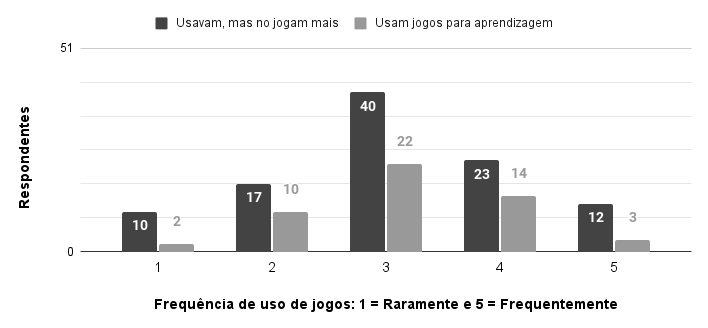
\includegraphics[keepaspectratio=true,scale=0.6]{figuras/resultados/freq-jogo.png}
	\legend{Fonte: Própria Autoria}
	\label{Fig:freq-jogo.png}
\end{figure}

Em relação à frequência de uso de jogos pode-se notar que a maioria se concentra num uso mediano de jogos para aprendizagem, tanto aqueles que usavam e deixaram de jogar, quanto dos que ainda usavam jogos para aprendizagem. Isto reforça a ideia de que o perfil dos jogadores aqui analisados tende usar jogos que não demandem muito tempo para que o objetivo de estudo do usuário seja alcançado.

Ainda foi possível identificar alguns jogos para aprendizagem, os quais os respondentes usaram. A Figura \ref{Fig:jogo-cit.png} apresenta estes jogos citados pelos respondentes. % Jogos Citados O02.1.3; O02.2.3

\begin{figure}[htbp]
	\centering
	\caption{Jogos para aprendizagem citados pelos respondentes}
	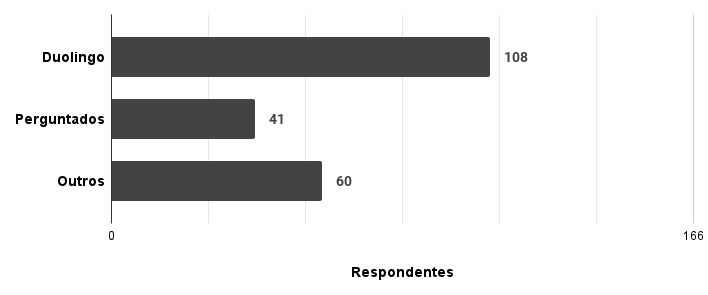
\includegraphics[keepaspectratio=true,scale=0.6]{figuras/resultados/jogo-cit.png}
	\legend{Fonte: Própria Autoria}
	\label{Fig:jogo-cit.png}
\end{figure}

Cada respondentes pôde citar um ou mais jogos, sendo que os mais mencionados foram o Duolingo com 108 (65\%) menções e o jogo Perguntados com 41 (25\%). Outros 48 jogos foram citados, porém alguns foram mencionados no máximo por 4 respondentes. São estes os demais jogos: Cake, Simpler, LingoDeer, Drops, Rosetta Stone, LingQ, Memrise, Mondly, MosaLingua, CodeCombat, Flexbox Froggy, Grid Garden, Grasshopper, Mimo, Regex Crossword, Scratch Jr, Scratch, Codecademy, SoloLearn, Programming Hub, SAE, URI, HackerRank, Coelho Sabido, CodyCross, Show do Milhão, Khan Academy, Cursa, Coursera, Memrise, Space Engine, Geoguessr
Lumosity, Elevate, Brain Test, EnigmaZ, Racha Cuca, Logic Gates, Mestre da Lógica, Peak, Math and Sorcery, Math Tricks, PhET Simulações Físicas, Habitica, Interland e Ouvido Perfeito.

Tanto o Duolingo quanto o Perguntados seguem um estilo de jogo de perguntas e respostas. Isto reflete num perfil de jogador que têm por preferência realizar essa prática simples de estudo respondendo questões, porém com elementos oriundos dos jogos que trazem uma experiência lúdica para dentro do estudo.

\section{Experiência do Jogador em Design}

% H01;

Quanto à experiência dos respondentes em design de interfaces e aplicativos de software, foi analisado qual o tipo de experiência eles tinham. Cada respondente apresentou se não tinha experiência em design ou se tinha um tipo ou vários. A Figura \ref{Fig:exp-design.png} apresenta os tipos de experiências.  

\newpage

\begin{figure}[htbp]
	\centering
	\caption{Experiência dos alunos com design}
	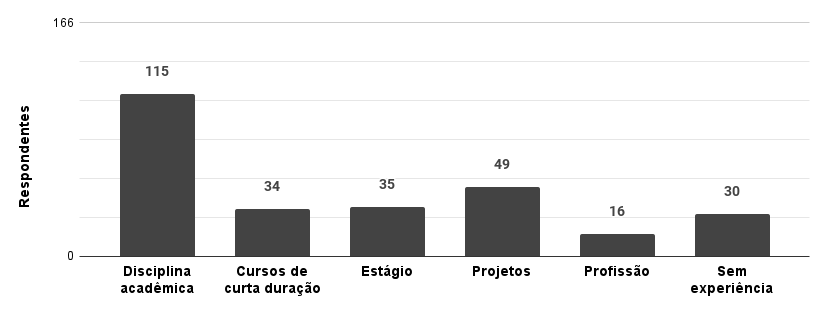
\includegraphics[keepaspectratio=true,scale=0.55]{figuras/resultados/exp-design.png}
	\legend{Fonte: Própria Autoria}
	\label{Fig:exp-design.png}
\end{figure}

Como pode ser observado na Figura \ref{Fig:exp-design.png}, 115 respondentes (69\%) tiveram pelo menos alguma experiência em design de interfaces em disciplinas acadêmicas; 34 respondentes (20\%) obtiveram pelo menos experiência com cursos de curta duração; 35 respondentes (21\%) ao menos tiveram experiência em design no estágio; 49 respondentes (29\%) conseguiram experiência em design ao menos com algum projeto pessoal, ou de pesquisa, ou de extensão, ou empresa júnior; e 16 respondentes (10\%) obtiveram ao menos experiência profissional com design de interfaces. Por fim, 30 respondentes (18\%) relataram não terem experiência em design.

Tendo em vista que a maioria dos respondentes tinham como parte de sua experiência em design, atividades acadêmicas, foi analisada esta experiência com relação à posição dos alunos quanto à disciplina de IHC. A Figura \ref{Fig:exp-design-disc.png} apresenta esta relação.


\begin{figure}[htbp]
	\centering
	\caption{Experiência dos alunos com design em relação a disciplina de IHC}
	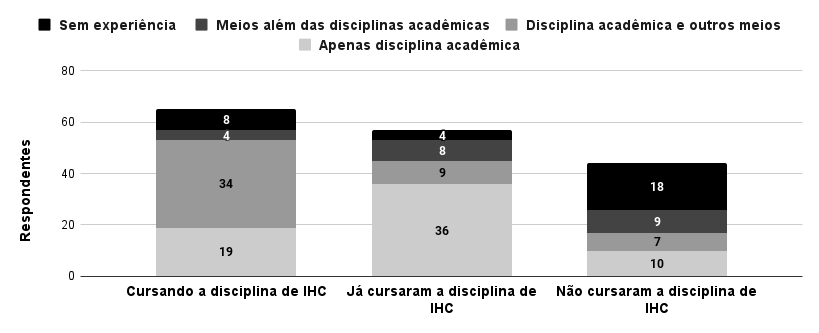
\includegraphics[keepaspectratio=true,scale=0.545]{figuras/resultados/exp-design-disc.png}
	\legend{Fonte: Própria Autoria}
	\label{Fig:exp-design-disc.png}
\end{figure}

Destes 115 respondentes que tiveram experiência em design através de disciplinas acadêmicas foi observado, que 65 tinham alguma experiência a mais com projetos, no estágio, atividade profissional ou em cursos complementares (soma da porção inferior de cada barra na Figura \ref{Fig:exp-design-disc.png}), sendo que 19 estavam cursando a disciplina; 36 já haviam feito a disciplina de IHC; e 10 ainda não haviam feito. Neste caso, existem 29 jogadores-alvo (19 cursando e 10 que não cursaram IHC), que poderiam usar um jogo para aprender ou avaliar algo em IHC e 36 que teriam ao menos o intuito de revisar o que aprenderam.

Já os outros 50 alunos, estes tinham experiência apenas com as disciplinas acadêmicas (soma da porção do meio-inferior de cada barra na Figura \ref{Fig:exp-design-disc.png}), sendo que 34 estavam cursando IHC; 9 já haviam feito a disciplina; e 7 não cursavam. Estes respondentes, por conta da experiência em IHC, talvez usariam este tipo de jogo apenas para aprender algo ou avaliar seu conhecimento sobre um assunto bem específico, algo inovador, ou mais aprofundado em IHC, porém poderia ser o caso de raramente ser para revisar um conteúdo mais básico. 

Observou-se que 21 respondentes não tinham experiência em design através de disciplinas acadêmicas (soma da porção do meio-superior de cada barra na Figura \ref{Fig:exp-design-disc.png}), mas sim por outros meios (cursos, estágio, projetos, profissão). Destes, 4 estavam cursando a disciplina de IHC; 8 já tinham cursado; e 9 ainda não haviam feito a disciplina. Sendo assim, são 13 os candidatos a terem uma experiência de um conhecimento formal sobre IHC (4 que estavam cursando e 9 que ainda não haviam cursado) e a partir disto serem potenciais usuário de um jogo para que possam aprenderem ou avaliar seu conhecimento em IHC. Já os outros 8, são possíveis usuários de jogos para pelo menos revisar algum conteúdo de IHC.

Do restante da amostra, 30 alunos não tinham tido experiência em design (soma da porção superior de cada barra na Figura \ref{Fig:exp-design-disc.png}), sendo que 8 estavam cursando; 4 consideraram não ter tido experiência em design mesmo tendo feito a disciplina de IHC; e 18 ainda não haviam feito a disciplina. São então 26 possíveis usuários de jogos para aprenderem algum conteúdo em IHC (8 que estavam cursando e 18 que ainda não haviam cursado).

Nesta análise é possível observar que 112 respondentes (67\%) tem um perfil caracterizado por suas motivações, relação com a disciplina de IHC e experiência com design que podem ser tidos como potenciais usuários de jogos para uma aprendizagem formal do conteúdo de IHC. Estes são formados por um público com pouco ou nenhum conhecimento sobre IHC, mas que deseja aprender um conteúdo novo com jogos ou ainda avaliar seu conhecimento. 

\section{Aspectos de Qualidade em Jogos para Aprendizagem}

Os respondentes ainda evidenciaram a importância de alguns aspectos dos jogos para aprendizagem. Estes foram identificados como requisitos de qualidade e experiência do jogador no trabalho de \cite{silva_sales_mendes2021}. Conforme foi descrito na metodologia, cada um destes aspectos foi classificado segundo a preferência dos respondentes, gerando uma pontuação que reflete a importância deles para os jogadores. Essa pontuação varia de 0 à 644.


\subsection{Requisitos de Qualidade}
%----------- RQ ------------
Os requisitos de qualidade são conhecidos também como requisitos não-funcionais ou ainda requisitos de restrição. Segundo SWEBOK \cite{swebok2014}, estes requisitos atuam para restringir uma solução de software, além de influenciarem na experiência do usuário. Na Tabela \ref{tab:req-pont} são apresentados os requisitos de qualidade analisados, já classificados em sua ordem de importância e suas respectivas pontuações.%Um destes que pode ser citado é a usabilidade, que segundo a \citeonline{ISO9126-1} é um requisito de qualidade de software.

% RE01
\begin{table}[htbp]
\centering
\caption{Classificação dos Requisitos de Qualidade Apreciados pelos Jogadores}
\label{tab:req-pont}
\begin{tabular}{clcl}
\hline
\multicolumn{1}{|c|}{\textbf{Classificação}} & \multicolumn{1}{l|}{\textbf{Requisito de Qualidade}}       & \multicolumn{1}{c|}{\textbf{Pontuação}}  \\ \hline
\multicolumn{1}{|c|}{01}                  & \multicolumn{1}{l|}{\textit{Design} do jogo atraente}               & \multicolumn{1}{c|}{564}           \\ \hline
\multicolumn{1}{|c|}{02}                  & \multicolumn{1}{l|}{Oferece \textit{feedback} ao jogador}           & \multicolumn{1}{c|}{553}           \\ \hline
\multicolumn{1}{|c|}{03}                  & \multicolumn{1}{l|}{Regras fáceis e claras de se entender} & \multicolumn{1}{c|}{544}                    \\ \hline
\multicolumn{1}{|c|}{04}                  & \multicolumn{1}{l|}{Facilidade em aprender a jogar}        & \multicolumn{1}{c|}{542}                    \\ \hline
\multicolumn{1}{|c|}{05}                  & \multicolumn{1}{l|}{Padrão de \textit{design} consistente}          & \multicolumn{1}{c|}{538}           \\ \hline
\multicolumn{1}{|c|}{06}                  & \multicolumn{1}{l|}{Fontes usadas serem fáceis de ler}     & \multicolumn{1}{c|}{522}                    \\ \hline
\multicolumn{1}{|c|}{07}                  & \multicolumn{1}{l|}{Facilidade em jogar}                   & \multicolumn{1}{c|}{513}                    \\ \hline
\multicolumn{1}{|c|}{08}                  & \multicolumn{1}{l|}{Acessibilidade}                        & \multicolumn{1}{c|}{506}                    \\ \hline
\multicolumn{1}{|c|}{09}                  & \multicolumn{1}{l|}{Uso adequado das cores}                & \multicolumn{1}{c|}{503}                    \\ \hline
\multicolumn{1}{|c|}{10}                  & \multicolumn{1}{l|}{Oferece pontos e recompensas}          & \multicolumn{1}{c|}{480}                    \\ \hline
\multicolumn{1}{|c|}{11}                  & \multicolumn{1}{l|}{Apresenta \textit{ranking} dos jogadores}       & \multicolumn{1}{c|}{404}           \\ \hline
\multicolumn{1}{|c|}{12}                  & \multicolumn{1}{l|}{Possui uma narrativa ou história}      & \multicolumn{1}{c|}{340}                    \\ \hline

\end{tabular}
\legend{Fonte: Adaptado de \cite{silva_sales_mendes2021}}
\end{table}

No trabalho de \citeonline{silva_sales_mendes2021} estes requisitos de qualidade para jogos de aprendizagem refletem os critérios, metas de usabilidade e até mesmo princípios de \textit{design} definidos na literatura por \citeonline{nielsen1994, ISO9126-1, Preece_Rogers_Sharp_2005, BarbosaEtAl2021}.

No caso, o ``Design Atraente'', foi o requisito de qualidade de maior importância apontado pelos respondentes. Este aspecto está relacionado à avaliação do usuário e sua satisfação quanto à identidade visual, o tema e combinação de elementos gráficos do jogo \cite{silva_sales_mendes2021}. Isto revela que mesmo em jogos com o propósito de aprendizagem e não de mero entretenimento, há a intenção dos usuários em ter um sentimento de satisfação e prazer em jogar, além do aprendizado em si. No caso, desejando ter uma experiência visual agradável enquanto jogam.

O segundo aspecto, ``Oferece \textit{feedback}'' está relacionado ao sistema digital constantemente apresentar ao usuário informações relevantes sobre as atividades e operações realizadas \cite{silva_sales_mendes2021}, dando assim uma visibilidade do status do sistema \cite{Preece_Rogers_Sharp_2005}. Isto acaba confortando o usuário, pois diminui as dúvidas e incertezas quanto ao que está acontecendo no sistema e o quanto ele está progredindo em seu objetivo de estudo com o jogo. 

Por exemplo, o jogo que mais se destacou nas citações dos respondentes, o Duolingo, tem uma dinâmica de \textit{feedbacks} interessante, pois ao acertar uma pergunta o jogador recebe uma mensagem de congratulação e tem um avanço na barra de progresso. Já quando o jogador erra a questão, ele recebe uma mensagem informando o erro e qual é a resposta correta. Em um jogo de aprendizagem essa dinâmica é interessante, pois o jogador mesmo errando aprende, diminuindo o sentimento de frustração e quando ele acerta o mesmo tem a percepção do seu progresso de estudo, o que pode influenciar na sensação de satisfação e confiança no jogo em sua proposta de ensino.

O terceiro aspecto, ``Regras Fáceis e Claras de se Entender'' é influenciado pelo aspecto ``Facilidade em aprender a jogar'' \cite{Petri_Wangenheim_2019}, quarto na classificação dos respondentes. Nesta classificação dos aspectos, eles distam de apenas 4 pontos. Dito isto, ao analisar tanto o julgamento dos respondentes, quanto o próprio conceito destes aspectos, percebe-se uma proximidade. 

Dentro dos critérios de usabilidade de \citeonline{nielsen1994} os aspectos ``Regras Fáceis e Claras de se Entender'' e ``Facilidade em aprender a jogar'' estão relacionados à ``facilidade de recordação'' e à ``facilidade de aprendizagem'' (facilidade de aprender a usar um sistema), respectivamente. Isto se reflete no tempo que o jogador gasta para aprender como funciona a mecânica e regras do jogo e o esforço cognitivo de se lembrar das regras durante o jogo \cite{silva_sales_mendes2021}. 

Jogos que tenham regras difíceis de memorizar e que tenham uma mecânica muito complexas podem acarretar no fracasso na execução das atividades propostas pelo jogo e acabar dificultando o aprendizado do jogador, que por sua vez gera frustração e até a desistência de usar o jogo. 

O ``Padrão de \textit{design} conscistente'', quinto aspecto de qualidade, mesmo estando 4 posições abaixo do ``Design Atraente'', é um aspecto que o influencia \cite{Petri_Wangenheim_2019}, pois ter um design padronizado e consistente e que seja atraente agrega mais ainda à experiencia do jogador. Isto estaria refletido num design com botões, cores, texto, imagens e entre outros elementos seguindo um tema, identidade visual ou guia de estilo. Além de influenciar na experiência visual do jogador isto acaba facilitando até mesmo a apresentação do conteúdo do jogo ao usuário \cite{silva_sales_mendes2021}, assim como no ``reconhecimento ao invés de memorização'' \cite{nielsen1994}.

O sexto aspecto, ``Fontes usadas serem fáceis de ler'' está relacionado à acessibilidade \cite{Petri_Wangenheim_2019}. Este aspecto é um elemento que se preocupa em não impor um obstáculo na leitura do jogador quanto ao conteúdo apresentado no jogo \cite{silva_sales_mendes2021}. O aspecto de ``padrão de \textit{design} conscistente'' acaba também estando relacionado a este \cite{Petri_Wangenheim_2019}.

A ``Facilidade em jogar'' por mais que esteja ligada ao aspecto ``Regras Fáceis e Claras de se Entender'' \cite{Petri_Wangenheim_2019}, se encontra a 4 posições abaixo quanto ao seu nível de importância. Este aspecto está relacionado a eficiência do jogador em operar este tipo de sistema digital, ou seja, está relacionado ao quão difícil ou fácil é jogar o jogo \cite{silva_sales_mendes2021}. 

Enquanto que para outros tipos de sistema digitais a facilidade em usá-los é algo fundamental, num jogo se ter certos níveis de dificuldade e obstáculos acaba refletindo em desafios ao jogador, que por sua vez pode ser instigado e motivado a jogar. Do contrário, um jogo sem muitos desafios pode se tornar monótono e assim o jogador perder o interesse no jogo.  

Em relação à ``Acessibilidade'', oitavo aspecto, já foi pontuado sobre o uso das fontes \cite{Petri_Wangenheim_2019}, porém ela envolve outros elementos. A acessibilidade além de se preocupar com elementos que não criem impedimentos na interação de usuários em geral com algum sistema digital, ela também contempla casos específicos de usuários com algum tipo de limitação, seja ela motora, visual, auditiva, cognitiva etc \cite[p. 48]{BarbosaEtAl2021}.

Outro elemento que envolve a acessibilidade e que está relacionado com o nono aspecto de qualidade aqui analisado, é o ``Uso adequado das cores'' \cite{Petri_Wangenheim_2019}. Este aspecto envolve o uso de cores significativas que não dificultem a leitura e a identificação de elementos na interface do jogo \cite{silva_sales_mendes2021}. Mais uma vez, este aspecto acaba tendo também uma relação com o aspecto ``padrão de \textit{design} conscistente'' \cite{Petri_Wangenheim_2019} 

O décimo, décimo primeiro e décimo segundo aspectos, ``Oferece pontos e recompensas'', ``Apresenta \textit{ranking dos jogadores}'' e ``Possui narrativa ou história'' são elementos específicos dos jogos \cite{silva_sales_mendes2021}. \citeonline{Vianna_Vianna_Medina_Tanaka_Krug_2013} vai tratar esses aspectos como artifícios orientados a constituir uma relação entre o objetivo do jogo, as regras, os \textit{feedbacks} oferecidos e a participação do jogador.

Oferecer pontos e recompensas pode ser uma forma de incentivar o jogador a executar as atividade propostas no jogo e conquistar uma meta em troca de algo (pontos, emblemas, títulos e recompensas). De certa forma isto é um tipo de \textit{feedback} positivo, que informa o jogador que ele está realizando as atividade corretamente, estimulando-o a progredir.

Já um \textit{ranking} entre os jogadores estimula a competitividade, podendo provocar os jogadores a se engajarem mais na proposta do jogo. Porém enquanto que pra alguns pode acarretar num sentimento de realização e maestria, pra outros pode gerar sentimentos negativos.

Por último, o fato do jogo ter uma história ou narrativa pode acabar envolvendo as pessoas fazendo com que elas se interessem e joguem. Uma narrativa pode gerar esse sentimento de propósito e missão, sentimento extrínseco a proposta central do jogo, mas que pode atrair certos tipos de jogadores. 

Com essa classificação percebe-se que em relação aos jogos para aprendizagem os usuários não se importam apenas em aprender algo ou ter seu conhecimento avaliado, mas desejam usar jogos desse tipo que sejam atraentes visualmente e que respondam quando interagirem ou realizarem alguma ação no jogo.

Três destes aspectos tiveram uma pontuação bem próxima, o que revela uma importância quase que equivalente entre eles. Os jogadores em sua classificação revelam que o importante é um jogo ter a mecânica e regras fáceis de serem entendidas e recordadas, ou seja, o usuário não quer ter que ficar relembrando ou consultando as regras ou precisar fazer tutorias para poder jogar, mas sim ser o mais simples e intuitivo possível. E quase com a mesma relevância o usuário se importa em o jogo ter um tema, uma composição harmoniosa e padronizada entre cores, fonte e elementos gráficos.

Com um pouco menos de relevância, mas ainda sim tidos como importantes, os jogadores-alvo revelam que se preocupam com aspectos de acessibilidade, de fontes fáceis de ler e cores adequadas, ou seja, eles têm uma preocupação com a forma com que o conteúdo e demais elementos do jogo são apresentados na interface. E próximos a estes a facilidade em jogar. Este aspecto ocupando a sétima posição pode demonstrar que os usuários desejam um jogo fácil mas com uma certa ``dose'' de desafio.

Os aspectos mais específicos de jogos receberam uma pontuação relativamente baixa, quando comparados aos outros aspectos. Entende-se que estes elementos de jogos para aprendizagem, que oferecem recompensas, apresenta ranking ou uma narrativa não tem tanta importância, mas sim podem ser consideradas opcionais.

Pôde ser observado nesta análise um perfil de preferências em relação a alguns elementos presentes em jogos para aprendizagem. Mesmo se tratando sobre os requisitos de qualidade foi possível observar desde já alguns sentimentos e emoções envolvidos com estes aspectos. A seguir são apresentadas com um pouco mais de detalhes as experiências esperadas pelos usuários ao jogarem esse tipo de jogo.

%----------- PX ------------
\subsection{Experiências de Jogador}

Conforme citado por \citeonline[p 47]{BarbosaEtAl2021}, a experiência do jogador é descrita como a qualidade das interações jogador-jogo. Na Tabela \ref{tab:exp-pont} são apresentadas as experiências esperadas pelos jogadores, já classificadas em sua ordem de importância.

% E01
\begin{table}[htbp]
\centering
\caption{Classificação das Experiências Apreciada pelos Usuários}
\label{tab:exp-pont}
\begin{tabular}{clcl}
\hline
\multicolumn{1}{|c|}{\textbf{Classificação}} & \multicolumn{1}{l|}{\textbf{Experiência apreciada pelos jogadores}} & \multicolumn{1}{c|}{\textbf{Pontuação}} \\ \hline
\multicolumn{1}{|c|}{1}                   & \multicolumn{1}{l|}{Sentir satisfação em jogar e aprender}          & \multicolumn{1}{c|}{600}                   \\ \hline
\multicolumn{1}{|c|}{2}                   & \multicolumn{1}{l|}{Ter confiança de que aprenderei o conteúdo}     & \multicolumn{1}{c|}{558}                   \\ \hline
\multicolumn{1}{|c|}{3}                   & \multicolumn{1}{l|}{Perceber a relevância do conteúdo ensinado}     & \multicolumn{1}{c|}{554}                   \\ \hline
\multicolumn{1}{|c|}{4}                   & \multicolumn{1}{l|}{Me divertir}                                    & \multicolumn{1}{c|}{539}                   \\ \hline
\multicolumn{1}{|c|}{5}                   & \multicolumn{1}{l|}{Me sentir desafiado}                            & \multicolumn{1}{c|}{536}                   \\ \hline
\multicolumn{1}{|c|}{6}                   & \multicolumn{1}{l|}{Ter a atenção focada durante o jogo}            & \multicolumn{1}{c|}{528}                   \\ \hline
\multicolumn{1}{|c|}{7}                   & \multicolumn{1}{l|}{O jogo como o principal meio de aprendizagem}   & \multicolumn{1}{c|}{361}                   \\ \hline
\multicolumn{1}{|c|}{8}                   & \multicolumn{1}{l|}{Interagir com outros jogadores}                 & \multicolumn{1}{c|}{360}                   \\ \hline
                    
\end{tabular}
\legend{Fonte: Adaptado de \cite{silva_sales_mendes2021}}
\end{table}

No trabalho de \citeonline{silva_sales_mendes2021} é apresentada a relação entre as experiências de jogador identificadas na pesquisa e os aspectos de experiência desejáveis apresentados por \citeonline{Preece_Rogers_Sharp_2005}.

Nota-se que na classificação dos respondentes, a experiência de ``sentir satisfação em jogar e aprender'' é a experiência mais apreciada. Mais uma vez é reforçada a ideia de que existem motivações extrínsecas ao simples objetivo de aprender com o jogo. Na subseção anterior, durante a análise dos requisitos de qualidade foi possível perceber que cada um pode impactar na satisfação do jogador em aprender e jogar.  

Já o aspecto seguinte, o do jogador ``ter confiança de que será aprenderá o conteúdo'' retoma a ideia central dos jogos para aprendizagem, no qual o jogador aprenda o conteúdo proposto através de um jogo. O usuário deste tipo de jogo deseja ter um sentimento confiança que atingirá seu objetivo de estudo e não perderá seu tempo. Um requisito de qualidade, analisado na subseção anterior, que pode impactar nessa experiência é o do jogo ``oferecer \textit{feedbacks}''. 

Próximo a este aspecto há o desejo do jogador ``perceber a relevância do conteúdo ensinado''. Esta é uma expectativa importante do jogador, que deve ser refletida em elementos (requisitos) do jogo que ressaltem a qualidade do conteúdo disciplinar. Os aspectos de acessibilidade, uso adequado de cores e de fontes, são elementos do jogo que se não forem bem trabalhados podem dificultar a percepção do jogador quanto ao conteúdo e a proposta do jogo.

Em quarto lugar, de acordo com a classificação dos respondentes, a ``Diversão'' ainda é um sentimento apreciado pelos jogadores, mesmo não sendo o propósito central desse tipo de jogo. Tal como a diversão, em quinto lugar, é classificado o ``Desafio''. E em sexto lugar tem-se a ``Atenção focada durante o jogo''. A forma como estes elementos serão trabalhados num jogo é subjetiva e vai depender do perfil do jogador-alvo. 

Por exemplo, para alguns receber pontos, ter um ranking para comparar suas conquistas ou até mesmo ter uma história ou narrativa pode ser divertido e estimulador para alguns, mas para outros não. Da mesma forma, o nível de dificuldade de um jogo vai depender das habilidades e competências do jogador. E se o jogador vai ter sua atenção focada no jogo ou não, também vai depender de elementos que atendam um perfil de jogador-alvo, prendendo a sua atenção enquanto ele joga.

Em sétimo lugar encontra-se a percepção do jogador em ver ``o jogo como o principal meio de aprendizagem''. Neste caso, seria um dos extremos, seria o jogador tratar qualquer outro meio de aprendizagem (literatura base da disciplina, pesquisar na internet, sanar dúvidas com colegas e professor), como métodos excepcionais e usarem os jogos como forma de aprendizagem base. O outro extremo seria então apenas usar os jogos como ferramentas auxiliares de aprendizagem.

Por último, tem-se  o aspecto de ``Interagir com outros jogadores''. Isto pode ser refletido em desafios em grupos, competições, desafios, mercado de itens etc. Um aspecto de jogo que trabalha esse tipo de experiência é o jogo apresentar um ranking.

Percebe-se que segundo o perfil dos respondentes há um forte desejo pela satisfação não só de cumprir o objetivo de estudo, mas também do usuário desfrutar do jogo. Ainda assim o apreço do usuário em ter confiança que ele vai aprender e de que o conteúdo apresentado no jogo é relevante são fundamentais.

Diversão, desafio e atenção focada no jogo, por se tratarem de elementos bem dependentes do perfil do usuário, se faz necessário o conhecimento do estilo de jogo de preferência dos respondentes, uma lógica para se trabalhar o nível de desafio e técnicas para engajar e prender o foco do jogador.

Os dois últimos aspectos de qualidade relacionados às experiências, revelam que estes não foram muito relevantes para os respondentes. O jogo pode ser considerado apenas uma ferramenta auxiliar no processo de aprendizagem do aluno e não algo como o meio principal de estudo. E quanto à interação entre outros jogadores, os respondentes teriam mais afinidade em usar um jogo \textit{single player}, ou que pelo menos não tivessem atividades interativas relevantes, podendo estas serem opcionais no jogo.

Finalizada a apresentação e discussão sobre as características da amostra, são apresentadas no Capítulo \ref{chap:ele-pers} o elenco das personas deste trabalho. Estão abordadas a análise e discussão sobre a representatividade destas personas para com a amostra.




